% section | subsection | subsubsection | paragraph | subparagraph | verbatim | enumerate | item

% Just let it be an Article bro
\documentclass{article}

% Cover Metadata
\title{Developing AI Applications with Python and Flask}
\date{16 Oktober 2025}
\author{Maulana Hafidz Ismail}

% Equation Setup
\usepackage{amsmath}

% Image Setup
\usepackage{graphicx}
\usepackage{float}

% Link Setup
\usepackage{hyperref}

% Highlighting Setup
\usepackage{soul}
\usepackage{xcolor}
\sethlcolor{red!30}
\newcommand{\hlblue}[1]{\sethlcolor{cyan!30}\hl{#1}\sethlcolor{yellow}}

% Line Width
\sloppy
\setlength{\emergencystretch}{3em}
\hbadness=99999

% Code Syntax Setup
\usepackage{listings}
\usepackage{xcolor} % untuk warna
\lstset{
basicstyle=\ttfamily\small,
frame=single,
breaklines=true,
backgroundcolor=\color{gray!10},
keywordstyle=\color{blue},
commentstyle=\color{gray},
stringstyle=\color{red},
tabsize=2,
captionpos=b
}

% Start of the Article
\begin{document}

% Cover Page
\pagenumbering{gobble}
\maketitle
\newpage

% Table of Content Page
\tableofcontents
\newpage
\pagenumbering{arabic}

% Main Content
\section{Python Coding Practices and Packaging Concepts}
\subsection{Introduction}
Python dengan Flask adalah framework aplikasi web yang ringan dan fleksibel. Framework ini dikenal karena kesederhanaan, minimalis, dan kemudahan penggunaannya. Dirancang sebagai micro-framework yang menyediakan struktur ringan yang memudahkan pengembang membangun aplikasi web dengan cepat dan mudah, tanpa mengorbankan efisiensi dan kemampuan untuk meningkatkan skala proyek dari skala kecil ke aplikasi yang lebih besar dan kompleks.


\subsection{Python with Flask for large-scale development}
Flask adalah pilihan yang baik untuk aplikasi yang lebih kecil dan sederhana. Namun, istilah \verb|"mikro"| lebih berkaitan dengan apa itu Flask, alih-alih membatasi potensi skalabilitasnya. Flask dapat digunakan untuk sistem berskala besar dan aplikasi yang lebih kompleks dengan memperhatikan persyaratan dan batasan spesifik, perencanaan yang cermat, arsitektur yang baik, dan desain modular. Namun, Flask mungkin memerlukan upaya pengelolaan dan penskalaan yang lebih besar dibandingkan dengan kerangka kerja yang lebih tangguh dan kaya fitur.

Ekosistemnya yang kaya dan tangguh menyediakan alat, pustaka, dan fungsionalitas bagi pengembang untuk menangani tugas-tugas pengembangan web seperti perutean, penanganan permintaan, rendering templat, atau tugas serupa. Caching, penyeimbangan beban, replikasi, dan penyimpanan data Anda secara skalabel dapat membantu mencapai hasil yang optimal.


\subsection{Key Flask Capabilities}
\begin{itemize}
    \item \textbf{Extensibility and integration}: Flask dapat diperluas dan pengembang dapat menambahkan atau menghapus fitur yang memungkinkan kustomisasi. Flask terintegrasi secara mulus dengan pustaka dan kerangka kerja Python lainnya, memungkinkan pengembang untuk menggabungkan fungsionalitasnya dengan alat dan teknologi lain, sehingga meningkatkan kemampuannya.
    \item \textbf{Transparent documentation}: Dokumentasi Flask diterbitkan, memungkinkan pengembang untuk menggunakan API dan utilitas internalnya serta menemukan titik kait, penggantian, dan sinyal sesuai kebutuhan.
    \item \textbf{Custom implementation}: Kustomisasi bawaan dan kelas khusus dapat digunakan untuk hal-hal seperti objek permintaan dan respons. Kelas Flask memiliki banyak metode yang dirancang untuk subkelas. Anda dapat dengan cepat menambahkan atau menyesuaikan perilaku dengan membuat subkelas Flask dan menggunakan subkelas tersebut di mana pun Anda membuat instance kelas aplikasi.
    \item \textbf{Scaling considerations}: Anda dapat menggunakan penskalaan sedemikian rupa sehingga jika Anda menggandakan jumlah server, Anda akan mendapatkan kinerja sekitar dua kali lipat. Hanya ada satu faktor pembatas terkait penskalaan di Flask, yaitu penggunaan proksi lokal konteks. Proksi ini bergantung pada konteks yang dalam Flask didefinisikan sebagai thread, proses, atau greenlet. Jika server Anda menggunakan jenis konkurensi yang tidak berbasis thread atau greenlet, Flask tidak akan lagi dapat mendukung proksi global ini.
    \item \textbf{Modular development}: Carilah cara-cara agar proyek Anda dapat direfaktor menjadi kumpulan utilitas dan ekstensi Flask. Jelajahi berbagai ekstensi di komunitas dan cari pola untuk membangun ekstensi Anda sendiri jika Anda tidak menemukan alat yang dibutuhkan. Cara terbaik untuk meningkatkan alat untuk aplikasi yang lebih besar adalah dengan mendapatkan umpan balik dari pengguna.
\end{itemize}

\subsection{Real-world applications}

Saat ini, Python dengan Flask telah menjadi pilihan populer di kalangan perusahaan besar karena kesederhanaan, fleksibilitas, fleksibilitas, serta kemudahan pembelajaran dan penggunaannya. Desainnya yang minimalis dan sifatnya yang dapat dikustomisasi menjadikannya adaptif, efektif, dan andal untuk kebutuhan pengembangan web skala besar di berbagai industri dan sektor.

Beberapa perusahaan terkemuka, termasuk Netflix, Reddit, Lyft, LinkedIn, Pinterest, dan Uber, memanfaatkan Python dengan Flask dalam tumpukan teknologi mereka untuk layanan atau fungsionalitas backend tertentu. Python Flask menguntungkan perusahaan besar untuk berbagai tujuan seperti pengembangan API, layanan backend, pengembangan cepat, dan pembuatan prototipe, sementara ekstensibilitasnya memfasilitasi penambahan fungsionalitas ke dalam infrastruktur mereka. Hal ini menunjukkan bahwa Python Flask dapat menjadi bagian dari arsitektur yang skalabel jika dikombinasikan dengan strategi dan alat yang tepat.

\subsection{Fase dalam Application Development Lifecycle}
\begin{itemize}
    \item Requirement Gathering:

          Mengumpulkan kebutuhan dari pengguna, bisnis, dan teknis, pantangan (constraint).
          Contoh: Pengguna harus dapat melihat berbagai kamar dan fasilitas yang tersedia.
    \item Analysis:

          Menganalisis kebutuhan yang telah dikumpulkan untuk merancang solusi yang mungkin.
          Penting untuk mendokumentasikan semua pembaruan dalam desain.
    \item Design:

          Merancang solusi lengkap berdasarkan analisis yang dilakukan.
          Dokumentasi yang jelas dan ringkas diperlukan untuk fase berikutnya.
    \item Code and Test:

          Menggunakan dokumentasi desain untuk mengkode, menguji, dan merevisi aplikasi hingga memenuhi semua spesifikasi.
          Unit Testing: Pengujian pada level unit untuk memastikan setiap bagian kode berfungsi sesuai harapan.
    \item User and System Test:

          Pengujian dari sudut pandang pengguna dan pengujian sistem untuk memastikan aplikasi berfungsi dengan baik.
          Integration Testing: Memastikan semua program berfungsi setelah diintegrasikan.
          Performance Testing: Mengukur kecepatan, skalabilitas, dan stabilitas aplikasi.
    \item Production:

          Aplikasi tersedia untuk pengguna akhir.
          Aplikasi harus dalam keadaan stabil dan tidak mengalami perubahan besar.
    \item Maintenance:

          Aplikasi mungkin memerlukan pembaruan atau penambahan fitur baru.
          Fitur baru harus melalui semua fase sebelumnya sebelum diintegrasikan ke dalam aplikasi yang sudah ada.
\end{itemize}

\subsection{Praktik Terbaik dalam Pengkodean}
\begin{itemize}
    \item Menggunakan beberapa file untuk mengkode berbagai fungsionalitas.
    \item Membuat program pusat yang memanggil file-file individual untuk menjalankan fungsi tertentu.
\end{itemize}

\subsection{Web Applications}
\begin{itemize}
    \item Definisi: Web application adalah program yang disimpan di server jarak jauh dan diakses melalui internet menggunakan browser. Contoh: situs e-commerce, webmail.
    \item Komponen: Terdapat tiga komponen utama untuk memproses permintaan klien:
          \begin{itemize}
              \item Web Server: Mengelola permintaan yang diajukan.
              \item App Server: Menjalankan tugas yang diminta.
              \item Database: Menyimpan informasi yang diperlukan untuk menyelesaikan tugas.
          \end{itemize}
    \item Pengembangan: Kode ditulis untuk front-end menggunakan JavaScript, HTML, atau CSS, dan untuk back-end menggunakan Python, Java, atau Ruby.
\end{itemize}

\subsection{Keuntungan Web Applications}
\begin{itemize}
    \item Versi aplikasi yang sama dapat diakses oleh banyak pengguna secara bersamaan.
    \item Pengguna dapat menggunakan aplikasi dari berbagai platform (desktop, laptop, mobile).
    \item Aplikasi dapat diakses melalui browser tanpa perlu instalasi.
\end{itemize}

\subsection{Application Programming Interface (API)}
\begin{itemize}
    \item Definisi: API adalah komponen perangkat lunak yang memungkinkan dua aplikasi yang tidak terhubung untuk berkomunikasi. API memiliki aturan dan fungsi standar untuk menentukan data yang dapat diambil atau dimodifikasi.
    \item Contoh: Aplikasi cuaca yang meminta data dari weather API untuk memberikan ramalan cuaca.
    \item Arsitektur: API dapat dibangun menggunakan arsitektur seperti \textbf{Representational State Transfer (REST)} atau \textbf{Simple Object Access Protocol (SOAP)}.
    \item Manfaat API\@:
          \begin{itemize}
              \item Meningkatkan konektivitas antara aplikasi.
              \item Mendukung tindakan CRUD (Create, Read, Update, Delete).
              \item Bekerja dengan HTTP verbs seperti PUT, POST, DELETE, dan GET\@.
              \item Dapat disesuaikan karena berbasis HTTP\@.
          \end{itemize}
\end{itemize}

\subsection{Perbandingan Web Application dan APIs}
\begin{itemize}
    \item Semua web applications adalah APIs, tetapi tidak semua APIs adalah web applications.
    \item Contoh: Dalam layanan belanja e-commerce, browser bertindak sebagai API yang menghubungkan pengguna dengan web application.
\end{itemize}

\subsection{PEP-8 Guidelines untuk Keterbacaan Kode}
\begin{itemize}
    \item Indentasi: Gunakan empat spasi untuk setiap level indentasi. Ini penting karena editor teks dapat menginterpretasikan tab dengan cara yang berbeda, yang dapat menyebabkan kesalahan format.
    \item Baris Kosong: Gunakan baris kosong untuk memisahkan fungsi dan kelas. Ini membantu dalam memahami struktur kode dengan lebih baik.
\end{itemize}

\subsection{Konvensi Pengkodean untuk Konsistensi}
\begin{itemize}
    \item Fungsi Terpisah: Buat fungsi terpisah untuk blok kode yang lebih besar. Ini meningkatkan kecepatan eksekusi dan mendukung penggunaan kembali blok kode. Contoh sintaks:
          \begin{lstlisting}[language=Python, caption={}, captionpos=b]
            def function_one(a, b):
            return a + b
        \end{lstlisting}
    \item Penamaan Fungsi dan File: Gunakan huruf kecil dengan garis bawah (lowercase with underscores) untuk nama fungsi dan file. Ini mengikuti konvensi Python yang umum. Contoh: \verb|def calculate_area()|
    \item Penamaan Kelas: Gunakan CamelCase untuk nama kelas. Ini membantu membedakan antara kelas dan fungsi. Contoh: \verb|class MyClass|
    \item Konstanta: Gunakan huruf kapital dengan garis bawah untuk nama konstanta. Ini menunjukkan tujuan konstanta tersebut. Contoh: \verb|MAX_FILE_UPLOAD_SIZE|
\end{itemize}

\subsection{Analisis Kode Statis}
Analisis kode statis, atau analisis statis, adalah aktivitas verifikasi efisiensi kode aplikasi yang menganalisis kode sumber untuk kualitas, keandalan, dan keamanan tanpa mengeksekusi kode tersebut. Analisis kode statis merupakan bagian penting dari setiap siklus pengembangan aplikasi dan tersedia sebagai bagian dari berbagai kerangka kerja dengan Python.

Salah satu kerangka kerja yang paling populer adalah PyLint. PyLint pada dasarnya mengevaluasi kode berdasarkan kepatuhan terhadap panduan gaya pengkodean PEP8 dan menghasilkan komentar setiap kali menemukan masalah.

\begin{itemize}
    \item Static Code Analysis: Metode untuk mengevaluasi kode terhadap gaya dan standar yang telah ditentukan tanpa mengeksekusi kode. Ini membantu menemukan masalah seperti kesalahan pemrograman dan pelanggaran standar pengkodean Contoh alat: \textbf{PyLint} digunakan untuk memeriksa kepatuhan kode Python terhadap pedoman PEP-8.
\end{itemize}

\subsection{Definisi Unit Testing}
\begin{itemize}
    \item Unit Testing: Metode untuk memvalidasi apakah unit kode (bagian kecil dari aplikasi) berfungsi dengan baik.
\end{itemize}

\subsection{Proses Unit Testing}
\begin{itemize}
    \item Pengujian Dua Fase:
          Local Testing: Pengujian unit dilakukan di sistem lokal. Jika gagal, penyebabnya harus diidentifikasi dan diperbaiki.
    \item Server Testing:

          Setelah lulus pengujian lokal, unit diuji di server (misalnya, CICD server). Jika gagal, detail kegagalan akan diberikan untuk perbaikan.
\end{itemize}

\subsection{Membangun dan Menjalankan Unit Tests}
\begin{itemize}
    \item Unit Test Library:

          Digunakan untuk membuat unit tests. Ini adalah modul Python yang menyediakan kerangka kerja untuk pengujian.
    \item Penamaan File:

          File unit test harus memiliki awalan atau akhiran dengan kata \verb|"test"| untuk membedakannya dari file unit.
\end{itemize}

\subsection{Langkah-langkah Membuat File Unit Test}
\begin{itemize}
    \item Import Library:
          \begin{lstlisting}[language=Python, caption={}, captionpos=b]
            import unittest
        \end{lstlisting}
          unittest: Library Python untuk membuat dan menjalankan unit tests.
    \item Import Fungsi yang Diuji:
          \begin{lstlisting}[language=Python, caption={}, captionpos=b]
            from mymodule import square, doubler
        \end{lstlisting}
    \item Membangun Kelas Unit Testing:
          \begin{lstlisting}[language=Python, caption={}, captionpos=b]
            class TestMyModule(unittest.TestCase):
        \end{lstlisting}
          TestMyModule: Kelas yang digunakan untuk mengelompokkan unit tests. Harus mewarisi dari unittest.TestCase.
    \item Membuat Fungsi Test:
          \begin{lstlisting}[language=Python, caption={}, captionpos=b]
            def test_square(self):
            self.assertEqual(square(2), 4)
\end{lstlisting}
          assertEqual: Metode untuk membandingkan dua nilai. Jika nilai tidak sama, test akan gagal.
\end{itemize}

\subsection{Evaluasi Hasil Test}
\begin{itemize}
    \item Setelah menjalankan file test, output akan menunjukkan hasil test. Contoh output:
          \begin{itemize}
              \item Jika test berhasil: OK
              \item Jika test gagal: Menampilkan detail kegagalan, seperti:
          \end{itemize}
          \begin{lstlisting}[language=Python, caption={}, captionpos=b]
    Fail: test_square(_main_.TestMyModule)
    AssertionError: 8 is not equal to 4
\end{lstlisting}
\end{itemize}

\subsection{Kesimpulan terkait Unit Test}
Unit Testing adalah metode penting untuk memastikan bahwa setiap unit kode berfungsi dengan baik. Proses ini melibatkan pengujian di lingkungan lokal dan server, serta penggunaan library unittest untuk membangun dan menjalankan test. Output dari unit test memberikan informasi yang berguna untuk memperbaiki kesalahan sebelum aplikasi diterapkan.

\subsection{Module}
\begin{itemize}
    \item Definisi: Module adalah file \verb|.py| yang berisi definisi Python, pernyataan, fungsi, dan kelas yang dapat diimpor ke dalam skrip lain.
    \item Contoh Sintaks:
          \begin{lstlisting}[language=Python, caption={}, captionpos=b]
    def square(number):
    return number ** 2
\end{lstlisting}
          Fungsi square ini mengembalikan kuadrat dari input.
\end{itemize}

\subsection{Package}
\begin{itemize}
    \item Definisi: Package adalah kumpulan dari beberapa modules dalam sebuah direktori yang memiliki file \verb|__init__.py|, yang membedakannya dari direktori biasa.
    \item Contoh Struktur:
          \begin{lstlisting}[language=Python, caption={}, captionpos=b]
    my_project/
    __init__.py
    module1.py
    module2.py
\end{lstlisting}
          File \verb|__init__.py | digunakan untuk menginisialisasi package.
\end{itemize}

\subsection{Library}
\begin{itemize}
    \item Definisi: Library adalah kumpulan dari packages atau bisa juga berupa satu package. Contoh library termasuk NumPy, PyTorch, dan Pandas. Catatan: Istilah package dan library sering digunakan secara bergantian.
    \item Contoh Struktur Library:
          \begin{lstlisting}[language=Python, caption={}, captionpos=b]
    my_library/
    __init__.py
    package1/
        __init__.py
        module1.py
        module2.py
    package2/
        __init__.py
        module3.py
        module4.py
    package3/
        __init__.py
        module5.py
    \end{lstlisting}
    \item Pengunaan:
          \begin{lstlisting}[language=Python, caption={}, captionpos=b]
    from my_library.package1 import module1
    \end{lstlisting}
\end{itemize}

\subsection{Langkah-langkah Membuat Package}
\begin{itemize}
    \item Buat folder dengan nama package.
    \item Buat file kosong \verb|__init__.py|.
    \item Buat modules yang diperlukan.
    \item Tambahkan kode dalam \verb|__init__.py| untuk merujuk ke modules yang diperlukan. Contoh kode dalam \verb|__init__.py|:
          \begin{lstlisting}[language=Python, caption={}, captionpos=b]
    from . import module1
    from . import module2
\end{lstlisting}
\end{itemize}

\subsection{Verifikasi Package}
Verifikasi dilakukan untuk memastikan package dapat diimpor tanpa error.

Langkah-langkah:
\begin{itemize}
    \item Buka terminal bash.
    \item Pastikan direktori sama dengan folder package.
    \item Jalankan Python dengan perintah python.
    \item Ketik \verb|import my_project| untuk memverifikasi.
\end{itemize}

\subsection{Menggunakan Package}
\begin{itemize}
    \item Definisi: Setelah package dibuat, Anda dapat menggunakannya dalam skrip lain jika folder package berada dalam direktori yang sama. Contoh Sintaks:
          \begin{lstlisting}[language=Python, caption={}, captionpos=b]
    from my_project.module1 import square, doubler
    from my_project.module2 import mean
    
    print(square(4))  # Output: 16
    print(doubler(4))  # Output: 8
    print(mean(2, 1, 3))  # Output: 2
\end{lstlisting}
\end{itemize}

\subsection{}
\begin{itemize}
    \item
\end{itemize}

% New Sec
\newpage

\section{Web App Deployment using Flask}
\subsection{Python Libraries}
\begin{itemize}
    \item Definisi: Python libraries adalah kumpulan alat yang menyediakan fungsi tertentu untuk mempermudah dan mempercepat tugas pemrograman.
    \item Contoh Libraries:
          \begin{enumerate}
              \item NumPy: Memfasilitasi perhitungan matematis yang kompleks.
              \item Pandas: Menawarkan kemampuan manipulasi dan analisis data.
              \item Matplotlib: Mempermudah visualisasi data.
              \item Requests: Menyederhanakan pengiriman HTTP requests.
              \item BeautifulSoup: Memudahkan pengambilan informasi dari halaman web.
              \item SQLAlchemy: Toolkit SQL dan alat Object-Relational Mapping (ORM) untuk manajemen database.
              \item PyTest: Framework pengujian yang memungkinkan pembuatan tes sederhana hingga kompleks.
          \end{enumerate}
\end{itemize}

\subsection{Frameworks}
\begin{itemize}
    \item Definisi: Framework adalah struktur yang telah ditentukan untuk pengembangan aplikasi, menyediakan pedoman dan struktur untuk menulis dan mengorganisir kode.
    \item Contoh Frameworks:
          \begin{enumerate}
              \item Django
              \item Flask
              \item Web2Py
          \end{enumerate}
\end{itemize}

\subsection{Manfaat Menggunakan Framework}
\begin{itemize}
    \item Menyederhanakan Proses Pengembangan: Dengan kode yang sudah ditulis sebelumnya, pengembang dapat menghemat waktu.
    \item Mempermudah Debugging: Framework menyediakan alat debugging yang sudah dibangun.
    \item Fungsionalitas Lebih dengan Kode yang Lebih Sedikit: Pengembang dapat memanfaatkan pustaka dan modul yang sudah ada.
    \item Efisiensi Manajemen Database: Framework dilengkapi dengan alat integrasi database.
    \item Keamanan: Memanfaatkan fitur keamanan yang sudah ada dalam framework.
\end{itemize}

\subsection{Perbedaan antara Libraries dan Frameworks}
\begin{itemize}
    \item Libraries: Kumpulan paket yang melakukan fungsi tertentu.
    \item Framework: Menyediakan alur dasar dan arsitektur aplikasi, memungkinkan pembangunan aplikasi secara keseluruhan.
\end{itemize}

\subsection{Definisi Flask}
Flash adalah sebuah micro framework untuk membuat aplikasi web dengan minimal dependencies. Flask tidak mengikat pengguna pada satu set alat tertentu.

\subsection{Instalasi Flask}
\begin{itemize}
    \item Untuk menginstal Flask, disarankan untuk membuat virtual environment menggunakan modul venv atau bin venv.
    \item Sintaks untuk menginstal Flask:
          \begin{lstlisting}[language=Python, caption={}, captionpos=b]
    pip install Flask==2.2.2
\end{lstlisting}
\end{itemize}

\subsection{Fitur Utama Flask}
\begin{itemize}
    \item Web Server: Menjalankan aplikasi dalam mode pengembangan.
    \item Debugger: Membantu dalam debugging aplikasi dengan menampilkan traceback interaktif di browser.
    \item Logging: Menggunakan logging standar Python untuk mencatat log aplikasi.
    \item Testing: Mendukung pengujian bagian-bagian aplikasi dengan framework seperti pytest dan coverage.
\end{itemize}

\subsection{Fitur Tambahan Flask}
\begin{itemize}
    \item Static Assets: Mendukung file statis seperti CSS, JavaScript, dan gambar.
    \item Jinja Templating: Menggunakan Jinja untuk membuat halaman dinamis.
    \item Routing: Mendukung URL dinamis dan pengalihan untuk layanan RESTful.
    \item Error Handling: Menyediakan penanganan kesalahan global di tingkat aplikasi.
    \item Session Management: Mendukung manajemen sesi pengguna.
\end{itemize}

\subsection{Ekstensi Komunitas Populer}
\begin{itemize}
    \item Flask-SQLAlchemy:

          Menambahkan dukungan untuk Object Relational Mapping (ORM) menggunakan SQLAlchemy, memungkinkan pengembang untuk bekerja dengan objek database dalam Python.
    \item Flask-Mail:

          Memungkinkan pengaturan server email SMTP untuk mengirim email dari aplikasi Flask.
    \item Flask-Admin:

          Memudahkan penambahan antarmuka admin ke aplikasi Flask, memungkinkan pengelolaan data dengan lebih mudah.
    \item Flask-Uploads:

          Menyediakan kemampuan untuk menambahkan pengunggahan file yang disesuaikan ke aplikasi Anda.
    \item Flask-CORS\@:

          Memungkinkan aplikasi Anda untuk menangani Cross-Origin Resource Sharing, sehingga permintaan JavaScript lintas domain dapat dilakukan.
    \item Flask-Migrate:

          Menambahkan dukungan untuk migrasi database menggunakan SQLAlchemy ORM, memudahkan pengelolaan perubahan skema database.
    \item Flask-User:

          Menyediakan manajemen pengguna, termasuk otentikasi dan otorisasi, serta fitur manajemen pengguna lainnya.
    \item Marshmallow:

          Menyediakan dukungan untuk serialisasi dan deserialisasi objek yang lebih luas, memudahkan konversi data antara format yang berbeda.
    \item Celery:
          Merupakan antrian tugas yang kuat untuk menjalankan tugas latar belakang sederhana hingga program multi-storage yang kompleks dan terjadwal.
\end{itemize}

\subsection{Perbandingan dengan Django}
\begin{itemize}
    \item Flask: Framework ringan dengan fleksibilitas tinggi, hanya menyediakan dependencies dasar.
    \item Django: Framework full-stack yang menyediakan semua yang diperlukan untuk membuat aplikasi lengkap, tetapi lebih opinionated.
\end{itemize}

\subsection{Membuat Aplikasi Flask}
\begin{itemize}
    \item Instalasi Flask: Pastikan Flask sudah terinstal sebelum membuat aplikasi.
    \item File Server: Buat file Python yang akan menjadi server, misalnya \verb|app.py|.
    \item Instansiasi Flask:
          \begin{lstlisting}[language=Python, caption={}, captionpos=b]
    from flask import Flask
    app = Flask(__name__)
\end{lstlisting}
    \item Dengan menggunakan \verb|__name__|, Flask dapat mengetahui lokasi file yang sedang dijalankan, sehingga dapat menemukan file-file yang diperlukan untuk aplikasi Anda, seperti template HTML dan file statis (CSS, JavaScript, gambar, dll.).
\end{itemize}

\subsection{Menambahkan Rute Pertama}
Gunakan dekorator \verb|(@app)| untuk mendefinisikan rute.
\begin{lstlisting}[language=Python, caption={}, captionpos=b]
@app.route("/")
def hello_world():
    return "<b>my first Flask application in action!</b>"
\end{lstlisting}
Route adalah jalur URL yang mengarah ke fungsi tertentu dalam aplikasi.

\subsection{Menjalankan Aplikasi}
Set variabel \verb|FLASK_APP| dan \verb|FLASK_ENV| sebelum menjalankan aplikasi.
\begin{lstlisting}[language=Python, caption={}, captionpos=b]
    export FLASK_APP=app.py
    export FLASK_ENV=development
\end{lstlisting}
\begin{itemize}
    \item \verb|FLASK_APP|: Menunjukkan nama file utama server.
    \item \verb|FLASK_ENV|: Menentukan lingkungan pengembangan atau produksi.
\end{itemize}

\subsection{Mengembalikan JSON}
Anda dapat mengembalikan objek yang dapat diserialisasi seperti dictionary.
\begin{lstlisting}[language=Python, caption={}, captionpos=b]
    return {"message": "Hello, World!"}
\end{lstlisting}
JSON adalah format data yang sering digunakan untuk pertukaran data antara server dan klien.

\subsection{Opsi Konfigurasi di Flask}
Variabel Konfigurasi adalah beberapa opsi konfigurasi yang dapat digunakan:
\begin{itemize}
    \item \verb|ENV|: Menunjukkan lingkungan (produksi atau pengembangan).
    \item \verb|DEBUG|: Mengaktifkan mode debug.
    \item \verb|SECRET_KEY|: Digunakan untuk menandatangani cookie sesi.
\end{itemize}

\subsection{Struktur Aplikasi}
\begin{itemize}
    \item Struktur Direktori Umum

          Berikut adalah contoh struktur direktori untuk aplikasi Flask:
          \begin{figure}[H]
              \centering
              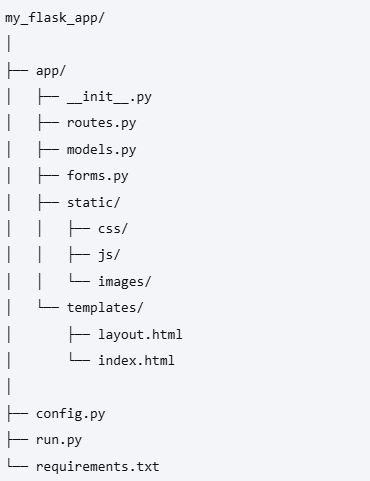
\includegraphics[width=0.8\textwidth]{flask_dir.png}
              \caption{Struktur Aplikasi Flask}
          \end{figure}

    \item Penjelasan Setiap Komponen
          \begin{itemize}
              \item \verb|my_flask_app/|: Ini adalah direktori utama untuk aplikasi Anda.
              \item \verb|app/|: Direktori ini berisi semua kode sumber aplikasi Flask Anda.
                    \begin{itemize}
                        \item \verb|__init__.py|: File ini digunakan untuk menginisialisasi aplikasi Flask dan mengatur konfigurasi. Di sini, Anda juga dapat mengimpor rute dan model.
                        \item \verb|routes.py|: File ini berisi semua rute (URL handlers) untuk aplikasi Anda. Di sinilah Anda mendefinisikan fungsi yang akan dijalankan ketika pengguna mengakses URL tertentu.
                        \item \verb|models.py|: File ini berisi definisi model data, biasanya digunakan dengan ORM (Object-Relational Mapping) seperti SQLAlchemy untuk berinteraksi dengan database.
                        \item \verb|forms.py|: File ini berisi definisi formulir yang digunakan dalam aplikasi, sering kali menggunakan Flask-WTF untuk menangani formulir dengan lebih mudah.
                        \item \verb|static/|: Direktori ini menyimpan semua file statis seperti CSS, JavaScript, dan gambar. File-file ini dapat diakses langsung oleh klien.
                        \item \verb|templates/|: Direktori ini berisi semua template HTML yang digunakan untuk merender halaman web. Flask menggunakan Jinja2 sebagai mesin templating, yang memungkinkan Anda untuk menyisipkan data dinamis ke dalam HTML\@.
                    \end{itemize}
              \item \verb|config.py|: File ini berisi konfigurasi aplikasi, seperti pengaturan database, kunci rahasia, dan opsi lainnya. Anda dapat mengatur berbagai konfigurasi untuk lingkungan pengembangan dan produksi di sini.
              \item \verb|run.py|: File ini adalah titik masuk untuk menjalankan aplikasi Flask. Anda dapat mengeksekusi file ini untuk memulai server Flask.
              \item \verb|requirements.txt|: File ini berisi daftar semua dependensi yang diperlukan untuk aplikasi Anda. Anda dapat menggunakan \verb|pip install -r requirements.txt| untuk menginstal semua paket yang diperlukan.
          \end{itemize}
\end{itemize}


% New Sec
\newpage

\section{Creating AI Application and Deploy using Flask}



% END
\end{document}